\chapter{Spezifische Ladung $e/m$ des Elektrons}
In diesem Teil des Praktikums soll die sogenannte spezifische Ladung des Elektrons bestimmt werden. Als spezifische Ladung bezeichnet man gemeinhin die Ladung pro Masse eines Teilchens. Diese Größe findet in mehreren Bereichen der Physik Anwendung, beispielsweise in der Massenspektrometrie, wo Analyten ionisiert und dann nach dem Kehrwert der spezifischen Ladung sortiert werden.

Hier ist allerdings die Möglichkeit wichtiger, über die Bestimmung des Verhältnisses $\frac{e}{m}$ auf die Masse des Elektrons zu schließen. Dies ist möglich, da zum Beispiel über den Millikan-Versuch die Elementarladung $e$ direkt bestimmt werden kann. 

Um mit den in diesem Versuch verfügbaren Aufbauten also die spezifische Ladung des Elektrons zu bestimmen, müssen zunächst einige mathematische Zusammenhänge für die involvierten physikalischen Größen bekannt sein:

Die Kräfte auf ein Elektron im elektromagnetischen Feld sind gegeben durch:
\begin{align}
	&\vec{F}=e\vec{E}&&\mathrm{Coulombkraft}\\
	&\vec{F}=-e\mu_r\mu_0\vec{v}\times\vec{H}=-e\vec{v}\times\vec{B}&&\mathrm{Lorentzkraft}
\end{align}
Nach Durchlaufen einer Potentialdifferenz U besitzt ein Elektron die potentielle Energie:
\begin{equation}
	W_{\mathrm{pot}}=eU
\end{equation}
Im Gegensatz dazu verrichtet die Lorentzkraft im Falle der Magnetostatik keine Arbeit am Teilchen. Aus der Energieerhaltung ergibt sich daher:
\begin{equation}
\label{eq:2} \frac{e}{m}=\frac{v^2}{2U}
\end{equation}
Da davon ausgegangen werden kann, dass die Bewegung des Elektrons in einer Ebene stattfindet, die senkrecht zu $\vec{B}$ ist, lässt sich weiterhin schreiben:
\begin{equation}
\label{eq:1} \frac{e}{m}=\frac{2U}{r^2B^2}
\end{equation}
\section{Vorbereitung}
\begin{enumerate}
	\item Leiten Sie Gleichung \eqref{eq:1} über den Zusammenhang zwischen Lorentz- und Zentripetalkraft her. Wie ist der Zusammenhang zwischen $e/m$ und den gemessenen Grössen $I,~U$ und $r$ ? Eliminieren Sie dabei die magnetische Induktion $B$ durch Verwendung des Kalibrierungsfaktors $K = B/I$ für die Helmholtzspulen! Wie kann bei konstantem Radius $r$ der Wert für $e/m$ graphisch ermittelt werden?
		\subitem Wie bereits oben klargestellt, kann man annehmen, dass $\vec{v}\perp\vec{B}$. Damit gilt:
		\begin{align*}
			\vec{v}\cdot\vec{B}&=0\\
			|\vec{v}\times\vec{B}|&=vB
		\end{align*}
		Somit gilt für die genannten Kräfte:
		\begin{align*}
			F_l&=F_z\\
			evB&=m\frac{v^2}{r}\\
			\frac{e}{m}&=\frac{v}{rB}\numberthis \label{eq:3}
		\end{align*}
		Mit Gleichung \eqref{eq:2} gilt:
		\begin{align*}
			\frac{v}{rB}&=\frac{v^2}{2U}\\
			v&=\frac{2U}{rB}
		\end{align*}
		Setzt man dies in \eqref{eq:3} ein, erhält man:
		\begin{displaymath}
			\frac{e}{m}=\frac{\frac{2U}{rB}}{rB}=\frac{2U}{r^2B^2}
		\end{displaymath}
		Nutzt man nun den Kalibrierungsfaktor $K=\frac{B}{I}$, so ergibt sich der Zusammenhang:
		\begin{displaymath}
			\frac{e}{m}=\frac{2U}{r^2K^2I^2}
		\end{displaymath}
		Hieraus sieht man sofort, dass e/m graphisch als Steigung eines $U-I^2-$Diagramms bzw. über den Achsenabschnitt eines $U-I-$Diagramms mit doppelt logarithmischer Skala bestimmt werden kann.
	\item Ein Elektron wird durch eine Spannung $U$ beschleunigt und unter einem Winkel $\alpha$ in ein Magnetfeld geschossen wie in Abb. \ref{fig:Abb5} gezeigt. Welche Bahn beschreibt das Elektron? Wie ändert sich der Bahnradius? Hinweis: Zerlegen Sie $\vec{v}$ in $v_\perp$ und $v_\parallel$ bzgl. $H$ und berechnen Sie daraus einerseits die Schraubenhöhe und andererseits auch die Umlaufzeit (Larmor-Frequenz).
	\begin{figure}[!h]
		\centering
		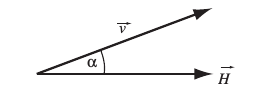
\includegraphics{emovement}
		\caption{Elektron im H-Feld}
		\label{fig:Abb5}
	\end{figure}
		\subitem Es gilt für die Geschwindigkeit:
		\begin{align*}
			v_\parallel&=v\cos\alpha\\
			v_\perp&=v\sin\alpha
		\end{align*}
		Hierbei leistet $v_\parallel$ keinen Beitrag zur Ablenkung durch die Lorentzkraft, da diese Komponente von $\vec{v}$ parallel zu $\vec{H}$ ist, das Kreuzprodukt verschwindet daher. Lediglich $v_\perp$ sorgt für eine Ablenkung des Elektrons, das im Folgenden eine Schraubenbahn beschreibt. Für die Schraubenhöhe $h$ gilt mit der Umlaufzeit $T$:
		\begin{displaymath}
			h= Tv_\parallel=Tv\cos\alpha
		\end{displaymath}
		Für den Radius der Kreisbahn ergibt sich aus dem Kräftegleichgewicht:
		\begin{align*}
			\mu_0eHv\sin\alpha&=m\frac{v^2\sin^2\alpha}{r}\\
			r&=\frac{mv\sin\alpha}{\mu_0eH}
		\end{align*}
		Daraus lässt sich nun die Umlaufzeit berechnen:
		\begin{displaymath}
			T=\frac{2\pi r}{v_\perp}=\frac{2\pi m}{\mu_0eH}
		\end{displaymath}
		Setz man dies in die obige Formel für die Ganghöhe ein, so kommt man schließlich zum Ergebnis:
		\begin{displaymath}
			h=\frac{2\pi mv\cos\alpha}{\mu_0eH}
		\end{displaymath}
	\item Wie kann man den Einfluss des Erdmagnetfelds auf die Elektronenbahn vermeiden?
		\subitem Am einfachsten kann dies bewerkstelligt werden, wenn man dafür sorgt, dass die Elektronen sich parallel zum Erdmagnetfeld bewegen. Ist dies nicht möglich, so kann Kompensation durch ein zum Erdmagnetfeld entgegengesetzt gleiches Feld erreicht werden.
\end{enumerate}
\section{Durchführung}
\subsection{Thomson-Röhre}
\begin{enumerate}
	\item Achten Sie darauf, dass während des gesamten Versuchs folgende Maxiamlwerte nicht überstiegen werden:
	\begin{itemize}
		\item Anodenspannung: 4 kV
		\item Spulenstrom: 0,9 A
	\end{itemize}
	\item Schließen Sie die Thomson-Röhre an das Hochspannungsnetzgerät an. Erhöhen Sie die Spannung, bis der Elektronenstrahl sichtbar ist (Raum muss abgedunkelt sein!!!).
	\item Legen Sie Spannung an die Spulen an und beobachten Sie den Strahlverlauf. Der Elektronenstrahlverlauf ist kreisförmig, die Ablenkung erfolgt in einer Ebene senkrecht zum elektromagnetischen Feld.
	\item Variieren Sie nun abwechselnd die Anodenspannung und den Spulenstrom, während Sie die andere Komponente konstant halten. Welche Auswirkung hat dies auf den Radius des Elektronenstrahls? Machen Sie sich die Zusammenhänge klar!
	\item Für die folgenden Schritte zur Bestimmung von $e/m$ stellen Sie nun einen Radius ein, der die aufgedruckte Skala schneidet.
	\item Bestimmung von $r$: Der Krümmungsradius $r$ des abgelenkten Elektronenstrahls lässt sich aus dem Austrittspunkt A mittels folgender Gleichung bestimmen:
	\begin{equation}
		r=\frac{80^2mm^2+e^2}{\sqrt{2}(80mm-e)}
	\end{equation}
	wobei sich $e$ direkt an der Skala ablesen lässt (siehe Abb \ref{fig:Abb6}).
	\begin{figure}[!h]
		\centering
		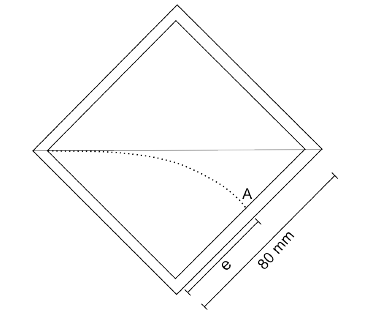
\includegraphics{emskizze}
		\caption{Bestimmung von r}
		\label{fig:Abb6}
	\end{figure}
	\item Bestimmung von $B$: Für die magnetische Flussdichte $B$ des Magnetfeldes bei Helmholtzgeometrie des Spulenpaars und dem Spulenstrom $I$ gilt:
	\begin{equation}
		B=\Big(\frac{4}{5}\Big)^\frac{3}{2}\cdot\frac{\mu_0\cdot n}{R}\cdot I=K\cdot I
	\end{equation}
	Der Kalibrier-Faktor für den angegebenen Aufbau ist $K=\SI{3,5}{\milli\tesla\per\ampere}$.
	\item Bestimmen Sie nun aus Spannung, Magnetfeld und Radius einen ersten Wert von $e/m$. Vergleichen Sie ihn mit dem akzeptierten Wert $e/m=\SI{1.76E11}{\ampere\second\per\kilogram}$. Falls Sie unvenünftig große Abweichungen feststellen, haben Sie wahrscheinlich irgendwo einen Fehler gemacht. Messen Sie erst weiter, wenn Sie diesen beseitigt haben.
	\item Nehmen Sie jetzt mehrere Wertepaare für $I$ und $U$ auf, wobei Sie darauf achten, den Radius $r$ konstant zu lassen.
	\item Machen Sie für Ihre Messungen eine genaue Fehlerbetrachtung, insbesondere unter Berücksichtigung der verschiedenen Wichtungen verschiedener Wertepaare. Beachten Sie dabei, dass auch die Bestimmung des Radius $r$ ungenau ist. Legen Sie diesen Fehler auf die Wertepaare $I$ und $U$ um. (Warum geht das?)
	\item Bestimmen Sie die spezifische Ladung $e/m$ eines Elektrons graphisch unter Berücksichtigung der Messfehler.
\end{enumerate}
\subsection{Doppelstrahlröhre}
\begin{enumerate}
	\item Achten Sie darauf, dass während des gesamten Versuchs folgende Maximalwerte nicht überstiegen werden:
	\begin{itemize}
		\item Plattenspannung: 45 V
		\item Spulenstrom: 0,4 A
	\end{itemize}
	\item Raumbeleuchtung abdunkeln, Heizspannung UF von 7 V einstellen und ca. 1 Minute warten bis sich die Temperatur der Heizung stabilisiert hat.
	\item Erhöhen Sie nun die Anodenspannung $U_A$ auf 100 V. Ohne anliegendes Magnetfeld erkennen Sie einen leuchtenden Strich.
	\item Stellen Sie den Spulenstrom $I_H$ so ein, dass ein geschlossener Kreis sichtbar wird. Beschreiben Sie, warum sich der anfänglich beobachtete Strich bei Erhöhung des Magnetfeldes dreht und zusammenzieht.
	\item Erhöhen Sie die Plattenspannung und beobachten Sie dessen Effekt auf den sichtbaren Elektronenkreis.
	\item Nachdem Sie sich mit dem Auswirkungen des Spulenstroms und der Plattenspannung auf die Elektronenbahn vertraut gemacht haben, variieren Sie nun beide Parameter um den Elektronenkreis möglichst genau an den Fluoreszenzschirm anzuschmiegen. Errechnen Sie unter Ausnutzung der Formel \eqref{eq:1} einen Wert für $e/m$. Schätzen Sie hierfür den Radius der Elektronenbahn ab (Tip: der Durchmesser des Glaskolbens beträgt 130 mm). Das Magnetfeld lässt sich durch die Helmholtz-Anordnung über folgende Beziehung bestimmen:
	\begin{displaymath}
		B^2=17,39\cdot 10^{-6}\cdot I_H^2
	\end{displaymath}
	\item Errechnen Sie $e/m$ für drei weitere Radien, wobei Sie die Plattenspannung konstant halten.
	\item Fehlerbetrachtung: Der kreisförmige Strahl ist sichtbar durch Photoemission. Warum ist der Fehler bei der Bestimmung von $e/m$ immer auf der negativen Seite?
\end{enumerate}